% ****** Start of file aipsamp.tex ******
%
%   This file is part of the AIP files in the AIP distribution for REVTeX 4.
%   Version 4.1 of REVTeX, October 2009
%
%   Copyright (c) 2009 American Institute of Physics.
%
%   See the AIP README file for restrictions and more information.
%
% TeX'ing this file requires that you have AMS-LaTeX 2.0 installed
% as well as the rest of the prerequisites for REVTeX 4.1
%
% It also requires running BibTeX. The commands are as follows:
%
%  1)  latex  aipsamp
%  2)  bibtex aipsamp
%  3)  latex  aipsamp
%  4)  latex  aipsamp
%
% Use this file as a source of example code for your aip document.
% Use the file aiptemplate.tex as a template for your document.
\documentclass[%
 aip,
 jmp,%
 amsmath,amssymb,
%preprint,%
 reprint,%
%author-year,%
%author-numerical,%
]{revtex4-1}

\usepackage{graphicx}% Include figure files
\usepackage{dcolumn}% Align table columns on decimal point
\usepackage{bm}% bold math
%\usepackage[mathlines]{lineno}% Enable numbering of text and display math
%\linenumbers\relax % Commence numbering lines
\usepackage{enumitem}
\usepackage{graphicx}
\usepackage{libertine}

\renewcommand{\vec}[1]{\bm{#1}}
\newcommand{\mat}[1]{\bm{#1}}
\newcommand{\vfun}[1]{\bm{#1}}
\newcommand{\set}[1]{\mathcal{#1}}
%\newcommand{\rset}{\mathbb{R}}
\newcommand{\term}[1]{\libertineSB{#1}\normalfont}
\newcommand{\norm}[1]{\|#1\|}
%\newcommand{\clsone}{$\mathcal{C}^1\ $}  % C1 function: continuously differentiable function
%\newcommand{\clstwo}{$\mathcal{C}^2\ $}  % C2 function: twice continuously differentiable function
%\newcommand{\lagr}{\mathcal{L}}

\newcommand{\R}[1]{\mathbb{R}^{#1}}    % real number set. R^n
\newcommand{\C}[1]{\mathcal{C}^{#1}}   % continuously differentiable. C1, C2, etc.
\renewcommand{\L}{\mathcal{L}}       % the Lagrangian
\renewcommand{\H}{\bm{\mathsf{H}}}   % Hessian matrix
\newcommand{\HL}{\bm{\mathcal{H}}}   % Hessian of Lagrangian
\newcommand{\N}{\mathcal{N}}    % the null space (kernel)
%\fontsize{10mm}{8mm}\selectfont

\begin{document}
\small

%\preprint{AIP/123-QED}

\title[ECON8013 - MATHEMATICAL TECHNIQUES FOR ECONOMICS]{KEYPOINT SUMMARY}% Force line breaks with \\


% \author{A. Author}
%  \altaffiliation[Also at ]{Physics Department, XYZ University.}%Lines break automatically or can be forced with \\
% \author{B. Author}%
%  \email{Second.Author@institution.edu.}
% \affiliation{
% Authors' institution and/or address%\\This line break forced with \textbackslash\textbackslash
% }%

% \author{C. Author}
%  \homepage{http://www.Second.institution.edu/~Charlie.Author.}
% \affiliation{%
% Second institution and/or address%\\This line break forced% with \\
% }%

% \date{\today}% It is always \today, today,
%              %  but any date may be explicitly specified

% \begin{abstract}
% An article usually includes an abstract, a concise summary of the work
% covered at length in the main body of the article. It is used for
% secondary publications and for information retrieval purposes.
% %
% Valid PACS numbers may be entered using the \verb+\pacs{#1}+ command.
% \end{abstract}

% \pacs{Valid PACS appear here}% PACS, the Physics and Astronomy
%                              % Classification Scheme.
% \keywords{Suggested keywords}%Use showkeys class option if keyword
%                               %display desired
\maketitle

% \begin{quotation}
% The ``lead paragraph'' is encapsulated with the \LaTeX\
% \verb+quotation+ environment and is formatted as a single paragraph before the first section heading.
% (The \verb+quotation+ environment reverts to its usual meaning after the first sectioning command.)
% Note that numbered references are allowed in the lead paragraph.
% %
% The lead paragraph will only be found in an article being prepared for the journal \emph{Chaos}.
% \end{quotation}

\section{LINEAR ALGEBRA BASICS}

\begin{enumerate}
    \item A nonempty set $\set{S} \in \R{n}$ is a \term{vector subspace} if
        \begin{enumerate}
            \item $\vec{0} \in \set{S}$, and
            \item $\vec{v_1} + \vec{v_2} \in \set{S}$, $\lambda \vec{v_1} \in \set{S}$  for all
                  $\vec{v_1}, \vec{v_2} \in \set{S}$.
        \end{enumerate}

    \item Let $\set{S}$ be a vector subspace of $\R{n}$. A group of vectors
    $\vec{v_1},\vec{v_2},\dots,\vec{v_m}$ are said to \term{span} $\set{S}$ if every vector in
    $\set{S}$ is a linear combination of $\vec{v_1},\vec{v_2},\dots,\vec{v_m}$.

    A group of vectors are called a \term{basis} of $\set{S}$ if they are
    \emph{linearly independent} and \emph{span} $\set{S}$.

    If $\set{S}$ has a basis consisting of $k$ vectors, it is said to be
    \emph{$k$-dimensional} and denoted as $\textrm{dim}\ S = k$.

        \begin{itemize}
            \item Any two bases of the same vector contains the \emph{same} number of vectors.
            \item Any combination of $n$ \emph{linearly independent} vectors in $\R{n}$ forms
                  a basis for $\R{n}$.
            \item Let $\set{S}$ be a subspace of a finite-dimensional vector space $\set{R}$.
                  If $\dim \set{S} = \dim \set{R}$, then $\set{S} = \set{R}$.
        \end{itemize}

    \item Given an $m \times n$ matrix $\mat{A}$. The subspace \emph{spanned} by the columns/rows of
          $\mat{A}$ is called the \term{column/row space} of $\mat{A}$.

    The dimension of the column/row space of $\mat{A}$ is called the \term{column/row rank} of $\mat{A}$.
        \begin{itemize}
            \item The column and row space are not the same if $m \neq n$.
            \item The column and row rank of a matrix are aways equal.
        \end{itemize}

    The solutions of the system $\mat{A}\vec{x} = \vec{0}$ form a vector space called the
    \term{null space (kernel)} of $\mat{A}$.

    \item \term{Fundamental Theorem of Linear Algebra}: For any $m \times n$ matrix $\mat{A}$
    $$ \dim Ker(\mat{A}) + rank(\mat{A}) = n$$

    \item Equivalent conditions for an $n \times n$ matrix $\mat{A}$ to be \term{invertible}:
        \begin{enumerate}
            \item $\mat{A}$ has $n$ row-leading $1$s in \emph{reduced row echelon form};
            \item The equation $\mat{A}\vec{x}=\vec{0}$ has only \emph{trivial solution} $\vec{x}=\vec{0}$;
            \item The columns of $\mat{A}$ are \emph{linearly independent};
            \item The columns of $\mat{A}$ form a basis for $\R{n}$;
            \item The rank of $\mat{A}$ is $n$;
            \item The kernel of $\mat{A}$ has $0$ dimension;
            \item The eigenvalues of $\mat{A}$ does not contain $0$;
            \item The \emph{determinant} of $\mat{A}$ is not $0$.
        \end{enumerate}

    \item Vectors $\vec{v_1}, \dots, \vec{v_k}$ are \term{orthogonal} to each other if
          $\vec{v_i}\cdot\vec{v_j}=0$ for $i \neq j$, and are \term{orthonormal} to each other
          if they further satisfies $\norm{\vec{v_1}}=\dots=\norm{\vec{v_k}}$.

    A matrix $\mat{O}$ is an \term{orthogonal} matrix if $\mat{O}^T\mat{O}=I$. The columns
    (or rows) of an orthogonal matrix are orthonormal to each other.

\end{enumerate}


\section{EIGENVALUES AND MATRIX DIAGONALIZATION}

\begin{enumerate}
    \item Let $\mat{A}$ be an $n \times n$ square matrix, if there exists $\lambda \in \R{}$
          and nonzero $\vec{v} \in \R{n}$ such that $$ \mat{A} \vec{v} = \lambda \vec{v}$$
          $\lambda$ is an \term{eigenvalue} of $\mat{A}$, and $\vec{v}$ is an \term{eigenvector}
          of $\mat{A}$ corresponding to eigenvalue $\lambda$.

    The eigenvalues of $\mat{A}$ are the \emph{roots} of the \term{characteristic polynomial} of
    $\mat{A}$: $$ |\mat{A} - \lambda\mat{I}| = 0 $$

    The set of all eigenvectors corresponding to an eigenvalue $\lambda$ forms the \term{eigenspace}
    of $\lambda$.

        \begin{itemize}
            \item Eigenvalues associated with different eigenvalues are \emph{linearly independent}.
            \item Suppose $\lambda_1, \dots, \lambda_n$ are the eigenvalues of $\mat{A}$. Then,
                \begin{itemize}
                    \item $\sum_{i=1}^{n} \lambda_i = \sum_{i=1}^{n} a_{ii}$ (trace of $\mat{A}$);
                    \item $\Pi_{i=1}^{n} \lambda_i = |\mat{A}|$.
                \end{itemize}
        \end{itemize}

    \item The \term{algebraic multiplicity} of an eigenvalue $\lambda_i$ is its exponent in the
        characteristic polynomial. The \term{geometric multiplicity} of an eigenvalue
        $\lambda_i$ is the dimension of its eigenspace.
            \begin{itemize}
                \item Geometric multiplicity can \emph{never exceed} the algebraic multiplicity.
                \item If for every eigenvalue of matrix $\mat{A}$, the geometric multiplicity
                    equals the algebraic multiplicity, then $\mat{A}$ is \emph{diagonalizable}.
            \end{itemize}

    \item A matrix $\mat{A}$ is \term{diagonalizable} if there exist matrices $\mat{P}$ and $\mat{D}$
          where $\mat{D}$ is a \emph{diagonal matrix} such that
          $$ \mat{A} = \mat{P}\mat{D}\mat{P}^{-1}$$
            \begin{itemize}
                \item An $n \times n$ matrix $\mat{A}$ is diagonalizable \emph{if and only if} the dimension
                      of its eigenspace is equal to $n$, i.e. the eigenvectors of $\mat{A}$ form a basis for $\R{n}$.
                \item Sufficient condition for diagonalization: $\mat{A}$ is diagonalizable if it has $n$ \emph{distinct}
                      eigenvalues. However, the converse might be false.
                \item The kernel of $\mat{A}$ is the \emph{eigenspace} corresponding to eigenvalue $0$. Thus the rank of of
                      $\mat{A}$ is the number of its non-zero eigenvalues (counted by \emph{multiplicity}).
            \end{itemize}

\end{enumerate}



\section{SYMMETRIC MATRICES AND QUADRATIC FORMS}

\begin{enumerate}


    \item Matrix $\mat{A}$ is \term{symmetric} if $\mat{A}=\mat{A}^T$. For any symmetric matrix $\mat{A}$,
        \begin{enumerate}
            \item $\mat{A}$ has only \emph{real} eigenvalues;
            \item $\mat{A}$'s eigenvectors corresponding to distinct eigenvalues are \emph{orthogonal};
            \item $\mat{A}$ is diagonalizable with orthogonal matrices, i.e. there exists a \emph{real diagonal}
                  matrix $\mat{D}$ and an $orthogonal$ matrix $\mat{O}$ such that
                  $ \mat{A} = \mat{O}\mat{D}\mat{O}^{-1} $.
        \end{enumerate}

    \item Suppose $\vec{v_1}, \vec{v_2}, \dots, \vec{v_k}$ are linearly independent and span vector subspace $\set{S}$.
          A set of \emph{orthogonal} vectors $\vec{w_1}, \vec{w_2}, \dots, \vec{w_k}$ can be found that span the same
          vector subspace $\set{S}$ following the \term{Gram-Schmidt Orthogonalization Process}:
            \begin{itemize}
                \item $\vec{w_1} = \vec{v_1}$
                \item $\vec{w_2} = \vec{v_2} - \dfrac{\vec{w_1}\cdot\vec{v_2}}{\vec{w_1}\cdot\vec{w_1}}\vec{w_1}$
                \item $\vec{w_3} = \vec{v_3} - \dfrac{\vec{w_1}\cdot\vec{v_3}}{\vec{w_1}\cdot\vec{w_1}}\vec{w_1} -
                       \dfrac{\vec{w_2}\cdot\vec{v_3}}{\vec{w_2}\cdot\vec{w_2}}\vec{w_2}$, and so on.
            \end{itemize}

    \item Let $\mat{A}$ be an $n \times n$ \emph{symmetric} matrix, then $\mat{A}$ is:
        \begin{enumerate}
            \item \term{positive definite} if $\vec{x}^T \mat{A} \vec{x} > 0$ for all $\vec{x} \neq \vec{0}$,
            \item \term{negative definite} if $\vec{x}^T \mat{A} \vec{x} < 0$ for all $\vec{x} \neq \vec{0}$,
            \item \term{positive semidefinite} if $\vec{x}^T \mat{A} \vec{x} \geq 0$ for all $\vec{x} \neq \vec{0}$,
            \item \term{negative semidefinite} if $\vec{x}^T \mat{A} \vec{x} \leq 0$ for all $\vec{x} \neq \vec{0}$,
            \item \term{indefinite} if $\vec{x}^T \mat{A} \vec{x} > 0$ for some $\vec{x}$ and $< 0$ for some other $\vec{x}$.
        \end{enumerate}
        \begin{itemize}
            \item Definiteness of quadratic forms can be defined with non-symmetric matrices, but we do not
                  consider this case. The following theorems only hold for symmetric matrices.
            \item If a matrix is positive or negative definite, then it must be \emph{nonsingular}.

            % \item A symmetric matrix is \emph{positive (negative) definite} if and only if all of its
            % eigenvalues are strictly positive (negative); it is \emph{positive (negative) semidefinite}
            % if and only if all of its eigenvalues are \emph{non-negative (non-positive)}.

            % \item A symmetric matrix is \emph{positive definite} if an only if all of its leading principal
            % minors are positive; it is \emph{negative definite} if and only if all of its leading principal
            % minors of even order are positive and all of its \emph{leading principal minors} of odd order
            % are negative. If some $k$th order leading principle minors of a matrix is nonzero but does not
            % fit either of the above two sign patterns, then it is \emph{indefinite}.

        \end{itemize}

    \item Let $\mat{A}$ be a symmetric matrix. Then $\mat{A}$ is:
        \begin{enumerate}
            \item positive definite iff all its eigenvalues are $>0$;
            \item negative definite iff all its eigenvalues are $<0$;
            \item positive semidefinite iff all its eigenvalues are $\geq 0$;
            \item negative semidefinite iff all its eigenvalues are $\leq 0$;
            \item indefinite iff $\mat{A}$ has both positive eigenvalues and negative eigenvalues.
        \end{enumerate}

    \item Let $\mat{A}$ be a symmetric matrix, and $D_k$ be its \term{leading principal minor} of order $k$,
          $\Delta_k$ for any of its \term{principal minors} of order $k$. Then $\mat{A}$ is:
            \begin{enumerate}
                \item positive definite iff all $D_k > 0$;
                \item negative definite iff all $(-1)^k D_k > 0$;
                \item positive semidefinite iff all $\Delta_k \geq 0$;
                \item negative semidefinite iff all $(-1)^k \Delta_k \geq 0$;
                \item indefinite if $D_k \neq 0$ but does not fit into any of the above patterns.
            \end{enumerate}

    \item Let $\mat{A}$ be a symmetric matrix. The following statements are equivalent:
            \begin{enumerate}
                \item $\mat{A}$ is positive definite;
                \item There exists nonsingular matrix $\mat{B}$: $\mat{A} = \mat{B}^T \mat{B}$;
                \item There exists nonsingular matrix $\mat{Q}$: $\mat{Q}^T \mat{A} \mat{Q} = \mat{I}$.
            \end{enumerate}

\end{enumerate}




\section{SINGULAR VALUE DECOMPOSITION}

\begin{enumerate}

\item \term{Singular Value Decomposition}: Any $m \times n$ matrix $\mat{A}$ can be decomposed as
$$
    \underset{m \times n}{\mat{A}} =
        \underset{m \times m}{\mat{U}}\
        \underset{m \times n}{\mat{\Sigma}}\
        \underset{n \times n}{\mat{V}^T}
$$
where $\mat{\Sigma}$ is a \emph{diagonal} matrix, $\mat{U}$ and $\mat{V}$ are \emph{orthogonal} matrices.
The diagonal entries of $\mat{\Sigma}$ is called the \term{singular values} of $\mat{A}$.

    \begin{itemize}
        \item The two facts below are used to compute an SVD:
        \item $\mat{A}^T\mat{A} = \mat{V}\mat{\Sigma}^T\mat{\Sigma}\mat{V}^T$
        \item $\mat{A}\mat{V}=\mat{U}\mat{\Sigma}$
    \end{itemize}


\item Suppose $m \times n$ matrix $\mat{A}$ has SVD of $\mat{A}=\mat{U}\mat{\Sigma}\mat{V}^T$:
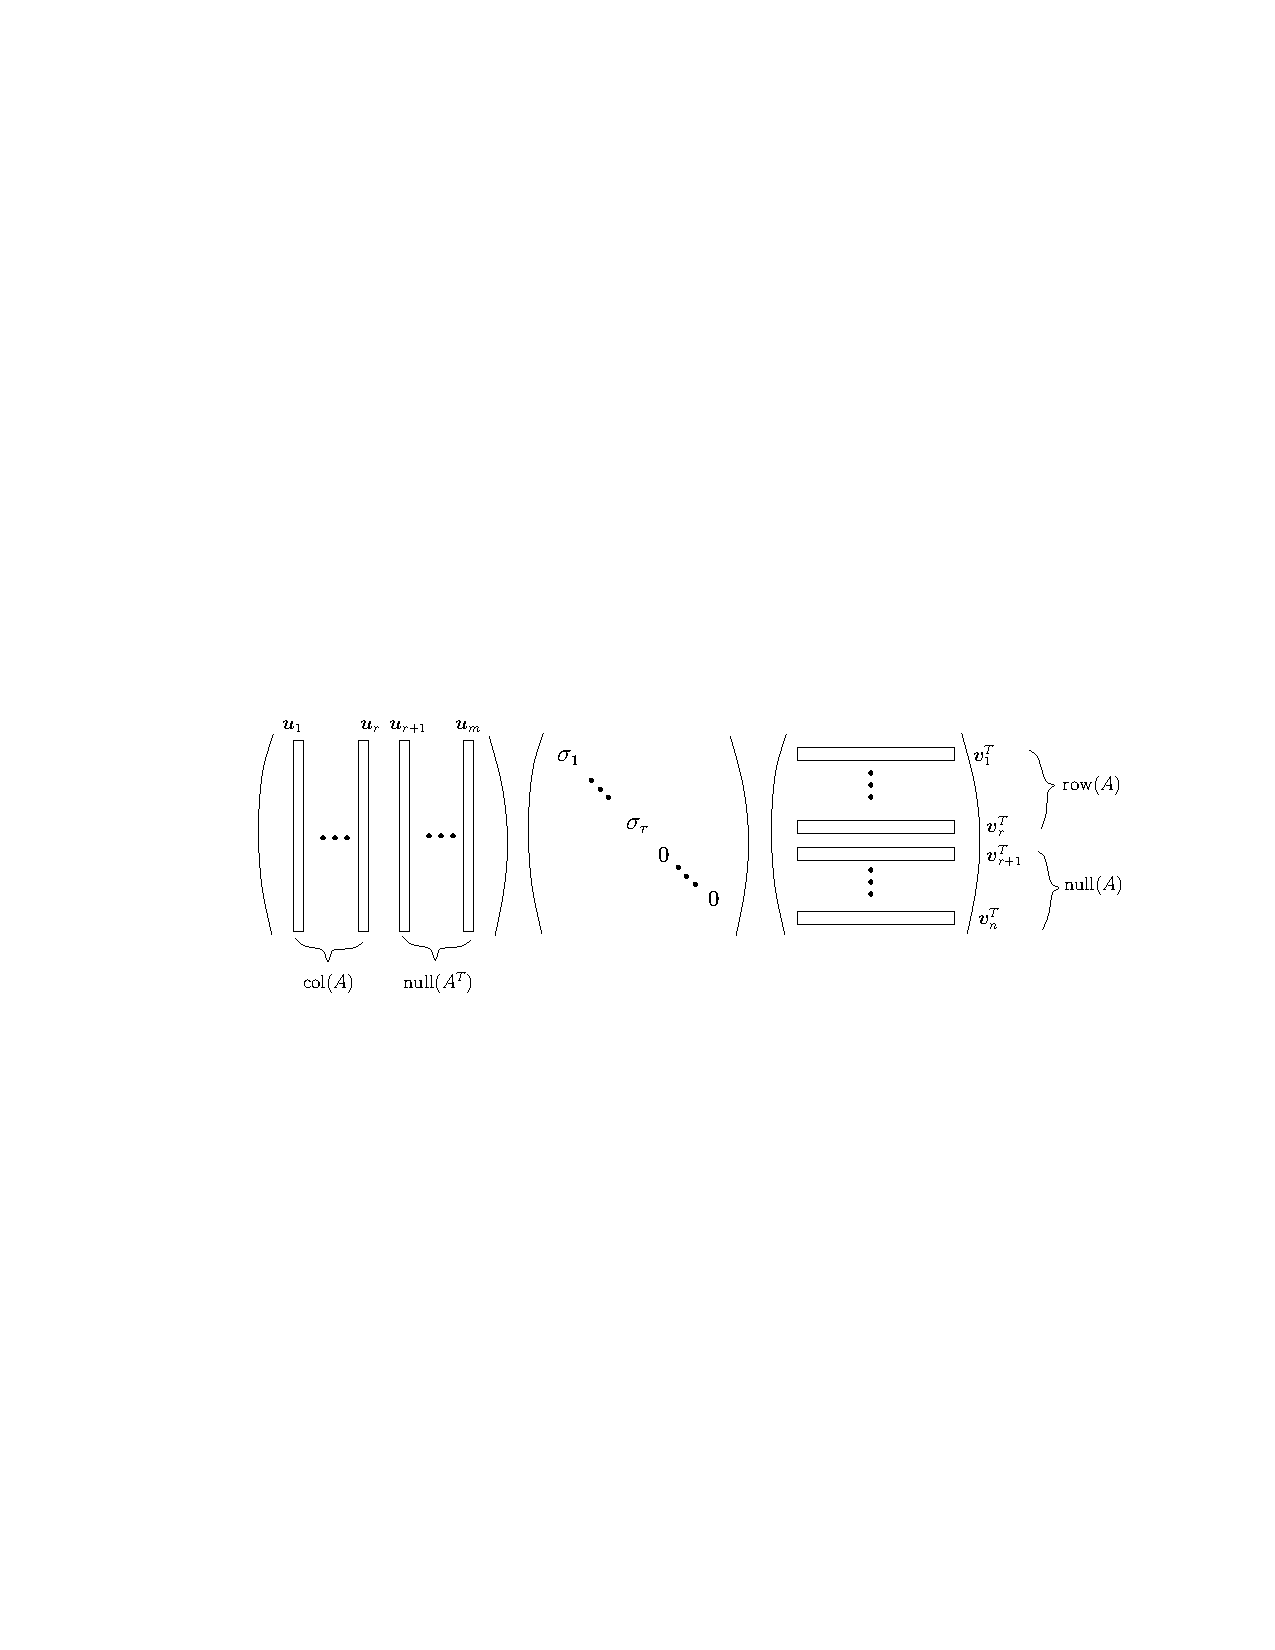
\includegraphics[scale=0.5]{svd.pdf}
Then the following properties hold:
    \begin{enumerate}
        \item $ rank(\mat{A}) = rank(\mat{\Sigma}) = r $;
        \item First $r$ columns of $\mat{U}$ are a basis of the column space;
        \item First $r$ columns of $\mat{V}$ are a basis of the row space;
        \item Last $n - r$ columns of $\mat{V}$ are a basis of $\N(\mat{A})$;
        \item Last ast $m - r$ columns of $\mat{U}$ are a basis of $\N(\mat{A^T})$.
    \end{enumerate}


\end{enumerate}

\section{COMPACT SETS AND EXTREME VALUE THEOREM}

\begin{enumerate}
\item A subset $\set{S} \subset \R{n}$ is an \term{open set} if for every $\vec{x} \in \set{S}$,
      there exists an open ball with $\epsilon > 0$ such that $B(\vec{x},\epsilon) \subset \set{S}$.
      A subset $\set{C} \subset \R{n}$ is a \term{closed set} if the complement of $\set{C}$ is open.
        \begin{itemize}
            \item All balls $B(\vec{x},\epsilon)$ are open sets.
            \item $\emptyset$ and $\mathbb{R}^n$ are both open and closed.
            % \item Any \emph{finite set} is both closed and compact.
        \end{itemize}

\item A \emph{closed} and \emph{bounded} subset of $\mathbb{R}^n$ is a \term{compact set}.

\item \term{Extreme Value Theorem}: Any \emph{continuous} function defined on a \emph{compact set}
       has a maximum and a minimum.

\end{enumerate}


\section{CALCULUS OF MULTIPLE VARIABLES}


\begin{enumerate}

\item \mbox{A vector-to-vector function $\vfun{f}: \R{n} \to \R{m}$ is defined as:}
$$\vfun{f}(\vec{x}) = (f_1(x_1,\dots,x_n), \dots, f_m(x_1,\dots,x_n)) $$
It is a bundle of $m$ functions from $\R{n}$ to $\R{}$.

\item Let $\vfun{f}: \R{n} \to \R{m}$, and $\vec{x^*} \in \R{n}$. $\vfun{f}$ is
      \term{differentiable} at $\vec{x^*}$ if there exists a \term{Jacobian matrix}
      $\mat{J}_{m \times n}$ such that
      $$ \vfun{f} (\vec{x^*} + \vec{h}) - \vfun{f} (\vec{x^*}) = \mat{J}\vec{h} + \vfun{r}(\vec{h}) $$
where $\vec{h} \in \R{n}$ and $\lim_{\norm{\vec{h}} \to 0} \frac{\norm{\vfun{r}(\vec{h})}}{\norm{\vec{h}}}=0$.

$\mat{J}$ is the \term{derivative} of $\vfun{f}$ at $\vec{x^*}$ and denoted as $D\vfun{f}(\vec{x^*})$.
Suppose function $\vfun{f}$ takes the form $$\vfun{f}(\vec{x}) = (f_1(x_1,\dots,x_n), \dots, f_m(x_1,\dots,x_n))$$

Then the Jocabian matrix of $\vfun{f}$ is calculated as
    \begin{equation*}
        D\vfun{f}(\vec{x}) =
            \begin{bmatrix}
                \frac{\partial f_1}{\partial x_1} & \frac{\partial f_1}{\partial x_2} & \dots & \frac{\partial f_1}{\partial x_n} \\
                \frac{\partial f_2}{\partial x_1} & \frac{\partial f_2}{\partial x_2} & \dots & \frac{\partial f_2}{\partial x_n} \\
                \vdots & \vdots & \ddots & \vdots \\
                \frac{\partial f_m}{\partial x_1} & \frac{\partial f_m}{\partial x_2} & \dots & \frac{\partial f_m}{\partial x_n} \\
            \end{bmatrix}
    \end{equation*}

\item The \term{gradient} of function $f(x_1,\dots,x_n)$ is defined as
$$\nabla f(\vec{x}) = \left[ \frac{\partial f}{\partial x_1}\ \frac{\partial f}{\partial x_2}\ \dots\ \frac{\partial f}{\partial x_n} \right] $$

The \term{directional derivative} of $f$ along $\vec{v}$ is defined as
$$ D_v f(\vec{x}) = (\nabla f(\vec{x})) \cdot \vec{v} $$
where $\vec{v}$ is a unit vector.
    \begin{itemize}
        \item $\nabla f(\vec{x})$ is a \emph{vector} while $D_v f(\vec{x})$ is a \emph{scalar}.
        \item The vector $\nabla f$ points to the direction along which $f$ \emph{increases most rapidly}.
        \item $D_v f(\vec{x})$ represents the \emph{instantaneous rate of change} of $f$ moving
              through $\vec{x}$ with a velocity specified by $\vec{v}$.
    \end{itemize}


\item Let $\mat{A}$ be a constant matrix, $\vec{a}$ be a constant vector. Let $\vfun{u}, \vfun{v}$ be
      vector functions and $\vec{u} = \vfun{u}(\vec{x})$, $\vec{v} = \vfun{v}(\vec{x})$.
        \begin{itemize}
            \item $\dfrac{\partial \vec{a} \cdot \vec{x}}{\partial \vec{x}} =
                   \dfrac{\partial \vec{a}^T  \vec{x}}{\partial \vec{x}} = \vec{a}^T $
            \item $\dfrac{\partial \mat{A}\vec{x}}{\partial \vec{x}} = \mat{A}$,
                  $\dfrac{\partial \vec{x}^T\mat{A}}{\partial \vec{x}} = \mat{A}^{T}$
            \item $\dfrac{\partial (\vfun{u} + \vfun{v})}{\partial \vec{x}} =
                   \dfrac{\partial \vfun{u}}{\partial \vec{x}} +
                   \dfrac{\partial \vfun{v}}{\partial \vec{x}} $
            \item $\dfrac{\partial (\vfun{u} \cdot \vfun{v})}{\partial \vec{x}} =
                   \vec{u}^T \dfrac{\partial \vfun{v}}{\partial \vec{x}} +
                   \vec{v}^T \dfrac{\partial \vfun{u}}{\partial \vec{x}} $
            \item $\dfrac{\partial \vfun{f}(\vfun{g}(\vfun{u}))}{\partial \vec{x}} =
                   \dfrac{\partial \vfun{f}(\vec{g})}{\partial \vec{g}}
                   \dfrac{\partial \vfun{g}(\vec{u})}{\partial \vec{u}}
                   \dfrac{\partial \vfun{u}}{\partial \vec{x}} $
            \item $\dfrac{\partial \vec{x}^T \mat{A} \vec{x}}{\partial \vec{x}} =
                   \vec{x}^T (\mat{A} + \mat{A}^T)
                   \underbrace{= 2\vec{x}^T \mat{A}}_{\mat{A} \textrm{ is symmetric}} $
        \end{itemize}


% \item \term{Chain Rule}: Let $F: \R{n} \to \R{m}$ and $G: \R{s} \to \R{n}$ be $\C{1}$  functions.
% Let $\vec{x^*} \in \R{s}$ and $G(\vec{x^*}) \in \R{n}$. The derivative for the \emph{composite function}
% $H = F \circ G$ is given by
% $$ D H(\vec{x^*}) = D F(G(\vec{x^*})) \cdot D G(\vec{x^*}) $$
% where the multiplication is \emph{matrix multiplication}.

\end{enumerate}


\section{IMPLICIT FUNCTION THEOREM}

\begin{enumerate}

\item \term{Implicit Function Theorem I}: Let $h(x_1, \dots, x_k, y)$ be a $\C{1}$ function around the point
      $\vec{x}^* = (x^*_1, \dots, x^*_k, y^*)$. Suppose $h(\vec{x}^*, y^*)=c$. If it satisfies
      $$ \frac{\partial h}{\partial y}(x^*_1, \dots, x^*_k, y^*) \neq 0 $$
Then there exits a $\C{1}$ function $y = g(\vec{x})$ defined on an open ball $B(\vec{x}^*,\epsilon)$ so that:
    \begin{enumerate}
        \item $y^* = g(\vec{x}^*)$;
        \item $g ( \vec{x}, g(\vec{x}) )=c$ for all $(\vec{x}) \in B(\vec{x}^*,\epsilon)$;
        \item $\left. \dfrac{\partial y}{\partial x_i}\right\rvert_{\vec{x}^*} =
               -\left.\dfrac{ \ \frac{\partial G}{\partial x_i}\ }{\ \frac{\partial G}{\partial y}\ }
               \right\rvert_{(\vec{x}^*, y^*)}$
    \end{enumerate}

\item \term{Implicit Function Theorem II}: Let $\vfun{f}: \R{m+n} \to \R{m}$ be $\C{1}$ where
      $\vfun{f}(\vec{y}, \vec{x}) = ( f_1(\vec{y}, \vec{x}), \dots, f_m(\vec{y}, \vec{x}) ) $.

Suppose $\vfun{f}(\vec{y}, \vec{x}) = \vec{c}$, or be written as
        \begin{align*}
            & f_1 ( y_1, \dots,  y_m, x_1, \dots, x_n ) = c_1 \\
            & \hspace{0.9in} \vdots \\
            & f_m ( y_1, \dots,  y_m, x_1, \dots, x_n ) = c_m
        \end{align*}

If the Jacobian matrix of $\frac{\partial \vfun{f}}{\partial \vec{y}}$ is \emph{nonsingular}, i.e.
    \begin{equation*}
        \left| \frac{\partial \vfun{f}}{\partial \vec{y} } \right| =
        \begin{vmatrix}
            \frac{\partial f_1}{\partial y_1} & \cdots & \frac{\partial f_1}{\partial y_m} \\
            \vdots & \ddots & \vdots \\
            \frac{\partial f_m}{\partial y_1} & \cdots & \frac{\partial f_m}{\partial y_m}
        \end{vmatrix} \neq 0
    \end{equation*}

Then there exists a $\C{1}$ function $\vec{y} = \vfun{g}(\vec{x})$ defined on an open ball
$B(\vec{x}^*, \epsilon)$ such that:
    \begin{enumerate}
        \item $\vec{y}^* = \vfun{g}(\mathbf{x^*})$;
        \item $\vfun{f}(\vfun{g}(\vec{x}), \vec{x}) = \vec{c}$ for all $\vec{x} \in B$;
        \item $\left.\dfrac{\partial \vec{y}}{\partial x_k}\right\rvert_{(\vec{y}^*, \vec{x}^*)}$ can be computed as below:
                \begin{equation*}
                  \begin{bmatrix}
                      \frac{\partial y_1}{\partial x_k} \\
                      \vdots \\
                      \frac{\partial y_m}{\partial x_k}
                  \end{bmatrix}
                  =-
                  \begin{bmatrix}
                        \frac{\partial f_1}{\partial y_1} & \cdots & \frac{\partial f_1}{\partial y_m} \\
                        \vdots & \ddots & \vdots \\
                        \frac{\partial f_m}{\partial y_1} & \cdots & \frac{\partial f_m}{\partial y_m} \\
                  \end{bmatrix}^{-1}
                  \begin{bmatrix}
                      \frac{\partial f_1}{\partial x_k} \\
                      \vdots \\
                      \frac{\partial f_m}{\partial x_k}
                  \end{bmatrix}
              \end{equation*}
    \end{enumerate}

\item \term{Inverse Function Theorem}: Let $\vfun{f}: \R{n} \to \R{n}$ (In order for a smooth map from
    $\R{n}$ to $\R{m}$ to be invertible, it is required $m=n$) be a $\C{1}$ function with
    $\vfun{f}(\vec{x}^*) = \vec{y}^*$. If $D\vfun{f}(\mathbf{x^*})$ is \emph{nonsingular},
    then there exists an open ball $B(\vec{x}^*,\epsilon)$ and an open set $\set{R}$ about $\vec{y}^*$
    such that $\vfun{f}$ is a \emph{one-to-one onto} map: $\set{B} \to \set{R}$, and the inverse map
    $\vfun{f}^{-1}: \set{R} \to \set{B}$ is also $\C{1}$ and further
    $$ (D\vfun{f}^{-1})(\vec{y}^*) = (D\vfun{f}(\vec{x}^*))^{-1} $$

\end{enumerate}


\section{CONVEXITY AND CONCAVITY}

\begin{enumerate}
    \item A set $\set{S}$ is called a \term{convex set} if for all $\vec{x}, \vec{y} \in \set{S}$ and $t \in [0,1]$,
    $t\vec{y} + (1-t)\vec{x} \in \set{S}$.

        \begin{itemize}
            \item The whole space $\R{n}$ is convex.
            \item Every vector subspace is also convex.
            \item The \emph{intersection} of convex sets is also a convex set.
            \item The set $\{ \vec{x} \in \R{n} : g_i(\vec{x}) \leq 0\ \textrm{for}\ i=1,2,\dots,n \}$ is
                  convex if $g_i$ is \emph{quasiconvex}.
            \item The set $\{ \vec{x} \in \R{n} : h_i(\vec{x}) = 0\ \textrm{for}\ i=1,2,\dots,n \}$ is
                  convex if $h_i$ is \emph{affine}.
        \end{itemize}

    \item Let $f$ be a function defined on a convex set $\set{S}$.
    $\forall \vec{x},\vec{y} \in \set{S}$ and $t \in [0,1]$,

    \mbox{$f$ is \term{convex} if $ f(t\vec{x} + (1-t)\vec{y}) \leq tf(\vec{x}) + (1-t)f(\vec{y}) $;}

    \mbox{$f$ is \term{concave} if $ f(t\vec{x} + (1-t)\vec{y}) \geq tf(\vec{x}) + (1-t)f(\vec{y}) $.}

    $f$ is \term{strictly convex/concave} if the strict inequalities hold whenever $\vec{x} \neq \vec{y}$
    and $t \in (0,1)$.

        \begin{itemize}[leftmargin=*]
            \item The sum of convex/concave functions are also convex/concave.
            \item In maximization problems, if the objective function is convex \emph{in its parameters},
                the value function is also convex.
            \item In minimization problems, if the objective function is concave \emph{in its parameters},
                the value function is also concave.
            \item If $f$ is a $\C{2}$ function, let $\H$ be its Hessian matrix, then:
                \begin{itemize}[leftmargin=*]
                    \item $f$ is convex $\Leftrightarrow$ $\H$ is positive semidefinite for $\forall \vec{x}$;
                    \item $f$ is concave $\Leftrightarrow$ $\H$ is negative semidefinite for $\forall \vec{x}$;
                    \item \mbox{$\H$ is positive definite for $\forall \vec{x}$ $\Rightarrow$ $f$ is strictly convex;}
                    \item \mbox{$\H$ is negative definite for $\forall \vec{x}$ $\Rightarrow$ $f$ is strictly concave.}
                \end{itemize}
                %\footnotesize{Note: the strict convexity (concavity) condition is sufficient but not necessary.}
        \end{itemize}


    \item Let $f$ be a function defined on a convex set $\set{S}$.
    $\forall \vec{x},\vec{y} \in \set{S}$ and $t \in [0,1]$,

    \mbox{$f$ is \term{quasiconvex} if $ f(t\vec{x} + (1-t)\vec{y}) \leq \max \{f(\vec{x}), f(\vec{y})\} $;}

    \mbox{$f$ is \term{quasiconcave} if $ f(t\vec{x} + (1-t)\vec{y}) \geq \min \{f(\vec{x}), f(\vec{y})\} $.}

    $f$ is \term{strictly quasiconvex/quasiconcave} if the strict inequality hold whenever $\vec{x} \neq \vec{y}$
    and $t \in (0,1)$.

        \begin{itemize}[leftmargin=*]
            \item A (strictly) convex/concave function is also (strictly) quasiconvex/quasiconcave.
            \item If $f$ is (strictly) quasiconvex/quasiconcave, and $g$ is strictly increasing,
                then $g \circ f$ is also (strictly) quasiconvex/quasiconcave.

            \item Convex sets and quasiconvex/quasiconcave functions:
                \begin{itemize}[leftmargin=*]
                    \item \term{Upper level set}:
                            $ \set{C}^{+}_{a} = \{ \vec{x}\in \set{S}: f(\vec{x}) \geq a \} $
                    \item \term{Lower level set}:
                            $ \set{C}^{-}_{a} = \{ \vec{x}\in \set{S}: f(\vec{x}) \leq a \} $
                    \item \mbox{$f$ is quasiconcave if \emph{every} upper level set of $f$ is convex;}
                    \item \mbox{$f$ is quasiconvex if \emph{every} lower level set of $f$ is convex.}
                \end{itemize}

            \item If $f$ is a $\C{2}$ function, let $\H$ be the Hessian for all $\vec{x}$, then
                \begin{itemize}[leftmargin=*]
                    \item \mbox{$f$ is quasiconvex $\Rightarrow$ $\H$ is positive semidefinite on $\N(\nabla f)$;}
                    \item \mbox{$f$ is quasiconcave $\Rightarrow$ $\H$ is negative semidefinite on $\N(\nabla f)$;}
                    \item \mbox{$\H$ is positive definite on $\N(\nabla f)$ $\Rightarrow$ $f$ is quasiconvex;}
                    \item \mbox{$\H$ is negative definite on $\N(\nabla f)$ $\Rightarrow$ $f$ is quasiconcave;}
                    \item In practice, let {\footnotesize $\mat{W}$} be a matrix whose columns are 
                        the basis of $\N(\nabla f)$. Then {\footnotesize $\H$} is negative (semi) definite on 
                        $\N(\nabla f)$ if and only if {\footnotesize $\mat{W}^T \H \mat{W}$} is a 
                        negative (semi) definite matrix.
                \end{itemize}

            \item If $f$ is a $\C{2}$ function, define the $r$-th order \term{Bordered Hessian} of $f$ as:
            \[
                \bar{\H} =
                \begin{bmatrix}
                    0    & f_1     & f_2     & \dots & f_r    \\
                    f_1  & f_{11}  & f_{12}  & \dots & f_{1r} \\
                    f_2  & f_{21}  & f_{22}  & \dots & f_{2r} \\
                    \vdots & \vdots & \vdots & \ddots& \vdots \\
                    f_r  & f_{r1}  & f_{r2}  & \dots & f_{rr} \\
                \end{bmatrix}
            \]
            Let $D_r$ be the determinant of its $r$-th order bordered Hessian, then
                \begin{itemize}[leftmargin=*]
                    \item $f$ is quasiconvex $\Rightarrow$ $D_k \leq 0$ for $\forall \vec{x} \in \set{S}$;
                    \item $f$ is quasiconcave $\Rightarrow$ $(-1)^k D_k \geq 0$ for $\forall \vec{x} \in \set{S}$;
                    \item $D_k < 0$ for $\forall \vec{x} \in \set{S}$ $\Rightarrow$ $f$ is quasiconvex;
                    \item $(-1)^k D_k > 0$ for $\forall \vec{x} \in \set{S}$ $\Rightarrow$ $f$ is quasiconcave.
                \end{itemize}
        \end{itemize}


\end{enumerate}



\section{OPTIMIZATION}

\begin{enumerate}

    \item \term{Existence of Solution}: Consider the optimization problem:
    \mbox{$ \max{f(\vec{x})}\ \textrm{s.t.}\ g_i(\vec{x}) \leq 0,\ h_i(\vec{x})=0 $.
    The solution \emph{exists} if:}
        \begin{enumerate}
            \item The feasible set is \emph{non-empty};
            \item The objective function is continuous;
            \item The constraint functions are continuous;
            \item The constraints are all \emph{weak inequalities};
            \item The feasible set is \emph{bounded}.
            \item[{}] \footnotesize{Sometimes solution still exists even if the feasible set is not bounded
                      if it can be proved that unbounded values are not optimal.}
        \end{enumerate}

    \item \term{Uniqueness of Solution}: Let $f: \set{S} \to \R{}$. If
        \begin{enumerate}
            \item $\set{S}$ is a \emph{convex set}, and
            \item $f$ is \emph{strictly quasiconcave};
        \end{enumerate}

        Then the \emph{global maximum} of $f$ on $\set{S}$ (if exists) is unique.

    \item \term{Unconstrained Optimization}: \\

    Let $f$ be a $\C{2}$ function. Consider the problem:
    $$ \underset{\vec{x} \in \R{n}}{\max} f(\vec{x}) $$

        \begin{itemize}[leftmargin=*]
            \item Necessary conditions for interior optimum: $$ \nabla f(\vec{x}^*) = 0 $$

            \item Sufficient conditions for local optimum: Let $\H$ be the Hessian matrix of $f$ at $\vec{x}^*$.
                \begin{itemize}[leftmargin=*]
                    \item \mbox{ $\vec{x}^*$ is a local maximizer $\Rightarrow$ $\H(\vec{x}^*)$ is negative semidefinite;}
                    \item \mbox{ $\H(\vec{x}^*)$ is negative definite $\Rightarrow$ $\vec{x}^*$ is a local maximizer;}
                \end{itemize}

            \item Sufficient conditions for global optimum:
                \begin{itemize}[leftmargin=*]
                    \item $f$ is \emph{concave} $\Rightarrow$ $\vec{x}^*$ is a global maximizer.
                \end{itemize}
        \end{itemize}

    \item \term{Constrained Optimization with Equality Constraints}: \\

    Let $f$, $h_1, \dots, h_k$ be $\C{2}$
        functions on $\R{n}$. Consider the problem:
            $$ \underset{\vec{x} \in \R{n}}{\max} f(\vec{x}) \textrm{ s.t. } h_j(\vec{x})=c_j $$

        \begin{itemize}[leftmargin=*]
            \item[{}] Let $\L (\vec{x}, \vec{\mu}) = f(\vec{x}) - \sum_{j=1}^{k} \mu_j (h_j(\vec{x}) - c_j)$.

            \item Necessary conditions for interior optimum:
                $$ \nabla_{\vec{x}} \L(\vec{x}^*, \vec{\mu}^*) = 0 $$
                $$ \forall j,\ h_j(\vec{x}^*) = c_j $$

            \item Constraint Qualification: The rows of the Jacobian $\bm{h}'(\vec{x}^*)$ are
                \emph{linearly independent}.

            \renewcommand{\HL}{\mat{\mathcal{H}}_{\vec{x}}}

            \item \mbox{Sufficient conditions for local optimum: Let $\HL(\vec{x}^*,\vec{\mu}^*)$ }
                be the Hessian of $\L$ with respect to $\vec{x}$ at $(\vec{x}^*,\vec{\mu}^*)$.
                \begin{itemize}[leftmargin=*]
                    \item $\vec{x}^*$ is a local maximizer $\Rightarrow$ $\HL$ is
                        negative semidefinite on $\N(\vfun{h}'(\vec{x}^*))$;
                    \item $\HL$ is negative definite on $\N(\vfun{h}'(\vec{x}^*))$
                        $\Rightarrow$ $\vec{x}^*$ is a local maximizer.
                    % \item In practice, let $\mat{W}$ be a matrix whose columns are basis of
                    %     $\N(\bm{h}'(\vec{x}^*))$. Then $\HL$ is negative (semi) definite on $\N(\bm{h}'(\vec{x}^*))$
                    %     if and only if $\mat{W}^T \HL \mat{W}$ is negative (semi) definite.
                    \item Border the $n \times n$ Hessian $\HL(\vec{x}^*,\vec{\mu}^*)$ with the $k \times n$ matrix $\vfun{h}'(\vec{x}^*)$:
                    \begin{equation*}
                        \qquad\qquad \begin{bmatrix}
                            0 & \cdots & 0 & | & \frac{\partial h_1}{\partial x_1} & \cdots & \frac{\partial h_1}{\partial x_n} \\
                            \vdots & \ddots & \vdots & | & \vdots & \ddots & \vdots \\
                            0 & \cdots & 0 & | & \frac{\partial h_k}{\partial x_1} & \cdots & \frac{\partial h_k}{\partial x_n} \\
                            \_\_ &  \_\_ &  \_\_ &  \_\_ &  \_\_ &  \_\_ &  \_\_  \\
                            \frac{\partial h_1}{\partial x_1} & \cdots & \frac{\partial h_k}{\partial x_1} & | & \frac{\partial^2 \L}{\partial x_1^2} & \cdots & \frac{\partial^2 \L}{\partial  x_n \partial x_1} \\
                            \vdots & \ddots & \vdots & | & \vdots & \ddots & \vdots \\
                            \frac{\partial h_1}{\partial x_n} & \cdots & \frac{\partial h_k}{\partial x_n} & | & \frac{\partial^2 \L}{\partial x_1 \partial x_n} & \cdots & \frac{\partial^2 \L}{\partial  x_n^2 } \\
                        \end{bmatrix}
                    \end{equation*}
                    Let $D_i$ be the $i$-th leading principal minor. If $(-1)^{k+i} D_i > 0$, then $\HL(\vec{x}^*,\vec{\mu}^*)$
                    is negative definite on $\N(\bm{h}'(\vec{x}^*))$.
                \end{itemize}

            \item Sufficient conditions for global optimum:
                \begin{itemize}[leftmargin=*]
                    \item \mbox{$\L$ is \emph{concave} $\Rightarrow$ $\vec{x}^*$ is a global maximizer 
                                s.t. $\vfun{h}(\vec{x}) = \vec{c}$}.
                    \item In particular, $f$ if concave and $\mu_j^* h_j$ is convex $\forall j$ $\Rightarrow$
                            $\vec{x}^*$ is a global maximizer s.t. $\vfun{h}(\vec{x}) = \vec{c}$.
                \end{itemize}
        \end{itemize}

    \item \term{Constrained Optimization with Inequality Constraints}: \\

    Let $f$, $g_1, \dots, g_m$, $h_1, \dots, h_k$
    be $\C{2}$ functions on $\R{n}$. Consider the problem:
        $$ \underset{\vec{x} \in \R{n}}{\max} f(\vec{x}) \textrm{ s.t. } g_i(\vec{x}) \leq b_i,\
        h_j(\vec{x})=c_i $$
        Define the Lagrangian:
        {\footnotesize
        $$ \qquad \L(\vec{x}, \vec{\lambda}, \vec{\mu}) = f(\vec{x}) -
            \sum_{i=1}^m \lambda_i (g_i(\vec{x})-b_i) -
            \sum_{j=1}^k \mu_j (h_j(\vec{x})-c_j)
        $$
        }
        \begin{itemize}[leftmargin=*]
            \item Necessary conditions for interior optimum:
                \begin{align*}
                    \qquad\qquad
                    & \nabla_{\vec{x}} \L(\vec{x}^*, \vec{\lambda}^*, \vec{\mu}^*) = 0 \\
                    & \forall i,\ g_i(\vec{x}^*) \leq b_i, \lambda_i \geq 0, \lambda_i (g_i(\vec{x}^*)-b_i)=0\\
                    & \forall j,\ h_j(\vec{x}^*) = c_j
                \end{align*}

            \renewcommand{\HL}{\mat{\mathcal{H}}_{\vec{x}}} 
            \item Sufficient conditions for local optimum: \\

            Suppose that $g_1, \dots, g_e$ are \emph{binding} at $\vec{x}^*$, and
            $g_{e+1}, \dots, g_m$ are non-binding. Let $\vfun{g}_E = (g_1, \dots, g_e)$.
            Let $\mat{C} = \begin{bmatrix}\vfun{g}_E'(\vec{x}^*) \\ \vfun{h}'(\vec{x}^*)\end{bmatrix}$.\\

            Let $\HL(\vec{x}^*, \vec{\lambda}^*, \vec{\mu}^*)$ be the Hessian of $\L$ with respect to $\vec{x}$ at
            $(\vec{x}^*, \vec{\lambda}^*, \vec{\mu}^*)$.

                \begin{itemize}[leftmargin=*]
                    \item $\vec{x}^*$ is a local maximizer $\Rightarrow$ $\HL$ is negative semidefinite on $\N(\mat{C})$;
                    \item $\HL$ is negative definite on $\N(\mat{C})$ $\Rightarrow$ $\vec{x}^*$ is a local maximizer.
                \end{itemize}

            \item Sufficient conditions for global optimum: $\vec{x}^*$ is a global maximizer if
                \begin{enumerate}
                    \item The feasible set is convex;
                    \item $f$ is concave, or
                    \item $f$ is quasiconcave and $\nabla f(\vec{x}^*) \neq 0$.
                \end{enumerate}
        \end{itemize}

    \item \term{Envelope Theorem (Unconstrained Version)}:
    $$  V(\vec{a}) = \underset{\vec{x}\in\R{n}}{\max} f(\vec{x}, \vec{a}) $$
    Assume that:
        \begin{enumerate}
            \item $\vec{x}^*(\vec{a}_0)$ is the \emph{unique} global maximum of $f(\vec{x}, \vec{a}_0)$;
            \item \mbox{$f(\vec{x}^*,\vec{a})$ is continuously differentiable in $\vec{a}$ at $(\vec{x}^*, \vec{a}_0)$;}
        \end{enumerate}
    Then $V(\vec{a})$ is differentiable at $\vec{a}_0$ and
    $$ \nabla_{\vec{a}} V(\vec{a}_0) = \nabla_{\vec{a}} f(\vec{x}^*, \vec{a}_0) $$
    {\footnotesize
        \begin{itemize}[leftmargin=*]
            \item Differentiability of $\vec{x}^*$, or differentiability of $f$ with respect to $\vec{x}$ are not required.
            \item This theorem also works for constrained optimization problems as long as no constraints depend on parameter $\vec{a}$.
        \end{itemize}
    }
    \item[{}] \term{Envelope Theorem (Constrained Version)}:
        $$\qquad V(\vec{a}) = \underset{\vec{x} \in \R{n}}{\max} f(\vec{x}, \vec{a})
            \textrm{ s.t. } g_i(\vec{x}, \vec{a}) \leq b_i, h_j(\vec{x}, \vec{a})=c_i
        $$
        Assume that:
            \begin{enumerate}
                \item $f, g_i, h_j$ all continuously differentiable with respect to both $\vec{x}$ and $\vec{a}$;
                \item $\vfun{x}^*(\vec{a}_0)$ satisfies the \emph{constraint qualification} and
                    is the \emph{unique} global constrained maximum;
                \item The set of binding inequalities remain \emph{unchanged} at optimality for near $\vec{a}_0$;
            \end{enumerate}
        Then $V(\vec{a})$ is differentiable at $\vec{a}_0$ and
        $$ \nabla_{\vec{a}} V(\vec{a}_0) = \nabla_{\vec{a}} \L(\vec{x}^*, \vec{\lambda}^*, \vec{\mu}^*, \vec{a}_0) $$

\end{enumerate}

\section*{} \vspace{5in} % end of document

\end{document}
